% Figure 1: Density Histogram of Normalized Attempts U = A / K^L
\begin{figure}[htbp]
\centering
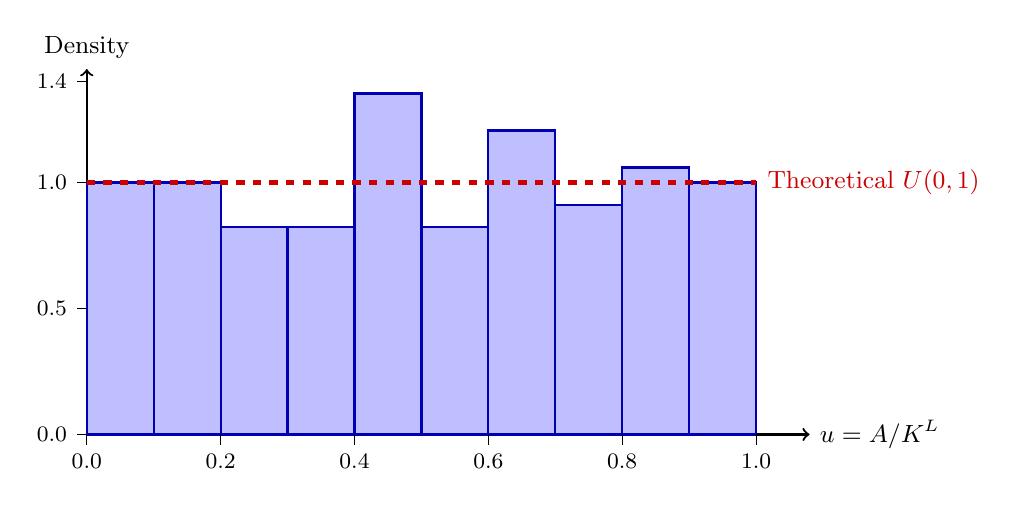
\begin{tikzpicture}[xscale=8.5, yscale=3.2]
  \draw[->, thick] (0,0) -- (1.08,0) node[right, font=\small] {$u = A / K^L$};
  \draw[->, thick] (0,0) -- (0,1.45) node[above, font=\small] {Density};
  \filldraw[fill=blue!25, draw=blue!70!black, thick] (0.0,0) rectangle (0.1,1.000);
  \filldraw[fill=blue!25, draw=blue!70!black, thick] (0.1,0) rectangle (0.2,1.000);
  \filldraw[fill=blue!25, draw=blue!70!black, thick] (0.2,0) rectangle (0.3,0.824);
  \filldraw[fill=blue!25, draw=blue!70!black, thick] (0.3,0) rectangle (0.4,0.824);
  \filldraw[fill=blue!25, draw=blue!70!black, thick] (0.4,0) rectangle (0.5,1.353);
  \filldraw[fill=blue!25, draw=blue!70!black, thick] (0.5,0) rectangle (0.6,0.824);
  \filldraw[fill=blue!25, draw=blue!70!black, thick] (0.6,0) rectangle (0.7,1.206);
  \filldraw[fill=blue!25, draw=blue!70!black, thick] (0.7,0) rectangle (0.8,0.912);
  \filldraw[fill=blue!25, draw=blue!70!black, thick] (0.8,0) rectangle (0.9,1.059);
  \filldraw[fill=blue!25, draw=blue!70!black, thick] (0.9,0) rectangle (1.0,1.000);
  \draw[red!80!black, ultra thick, dashed] (0,1.0) -- (1.0,1.0) node[right, font=\small] {Theoretical $U(0,1)$};
  \foreach \x in {0.0, 0.2, 0.4, 0.6, 0.8, 1.0}
    \draw (\x, 0) -- (\x, -0.04) node[below, font=\footnotesize] {\x};
  \foreach \y in {0.0, 0.5, 1.0, 1.4}
    \draw (0, \y) -- (-0.015, \y) node[left, font=\footnotesize] {\y};
\end{tikzpicture}
\caption{Empirical density of normalized attempts $u = A/K^L$ ($n = 340$) with the continuous uniform reference.}
\label{fig:norm_attempts_hist}
\end{figure}
